\documentclass[24pt,margin=1in,innermargin=-7.2in,blockverticalspace=-0.25in]{tikzposter}
\geometry{paperwidth=48in,paperheight=36in}
\usepackage[utf8]{inputenc}
\usepackage{csquotes}
% \usepackage[estonian]{babel}
\usepackage{amsmath}
\usepackage{amsfonts}
\usepackage{amsthm}
\usepackage{amssymb}
\usepackage{mathrsfs}
\usepackage{graphicx}
\usepackage{adjustbox}
\usepackage{multicol}
\usepackage{enumitem}
\usepackage{xcolor}
\usepackage[backend=biber,style=numeric]{biblatex}
\usepackage{unitartu-theme}
\usepackage{lipsum} 

\def\hide#1{\textcolor{white}{#1}}



\usepackage{mwe} % for placeholder images

\addbibresource{refs.bib}

% set theme parameters
\tikzposterlatexaffectionproofoff
\usetheme{UniTartuTheme}
\usecolorstyle{UniTartuStyle}

\usepackage[scaled]{helvet}
\renewcommand\familydefault{\sfdefault} 
\renewcommand{\vec}[1]{\bm{#1}}
\newcommand{\Tr}{\text{Tr}}
\usepackage[T1]{fontenc}

\title{DS 4420 Project Poster Template}
\author{\textbf{Eric Gerber}% \\ with \textbf{Nelson Guirado, Nikhil Bommareddy, Kaamil Thobani, Ryan Monahon}%\textsuperscript{2} % Add 2nd author
}
\institute{Northeastern University %and CSU Bakersfield\\
%\institute{\textsuperscript{1}Institute of Computer Science, University of Tartu\\
            %\textsuperscript{2}Institute of Mathematics, University of Tartu % Add 2nd author institute
            }
\titlegraphic{
\includegraphics[width=0.21\linewidth]{Monogram Wordmark_RGB_186+K.png}}

% begin document
\begin{document}
\maketitle
\centering
\begin{columns}
    \column{0.32}
    \block{Introduction/Abstract}{
         \lipsum[1]\\
         
    }
    \block{Motivation and Data}{
         \lipsum[2]

    \begin{multicols}{2}
        \begin{center}
        \vspace{1em}
        \begin{tikzfigure*}
            
\includegraphics[width=.75\linewidth]{Picture1}
        \end{tikzfigure*}
        \vspace{1em}
            
        \end{center}

        To the left here is an example image; maybe one used to illustrate the motivation of the project. Below, you might describe the data and give a couple basic EDA plots, or begin describing methodology.
    \end{multicols}

        \vspace{.5em}
        \lipsum[3]

         \begin{multicols}{2}
        \vspace{1em}
        \begin{tikzfigure}[Most players retire without reaching MLB.]
            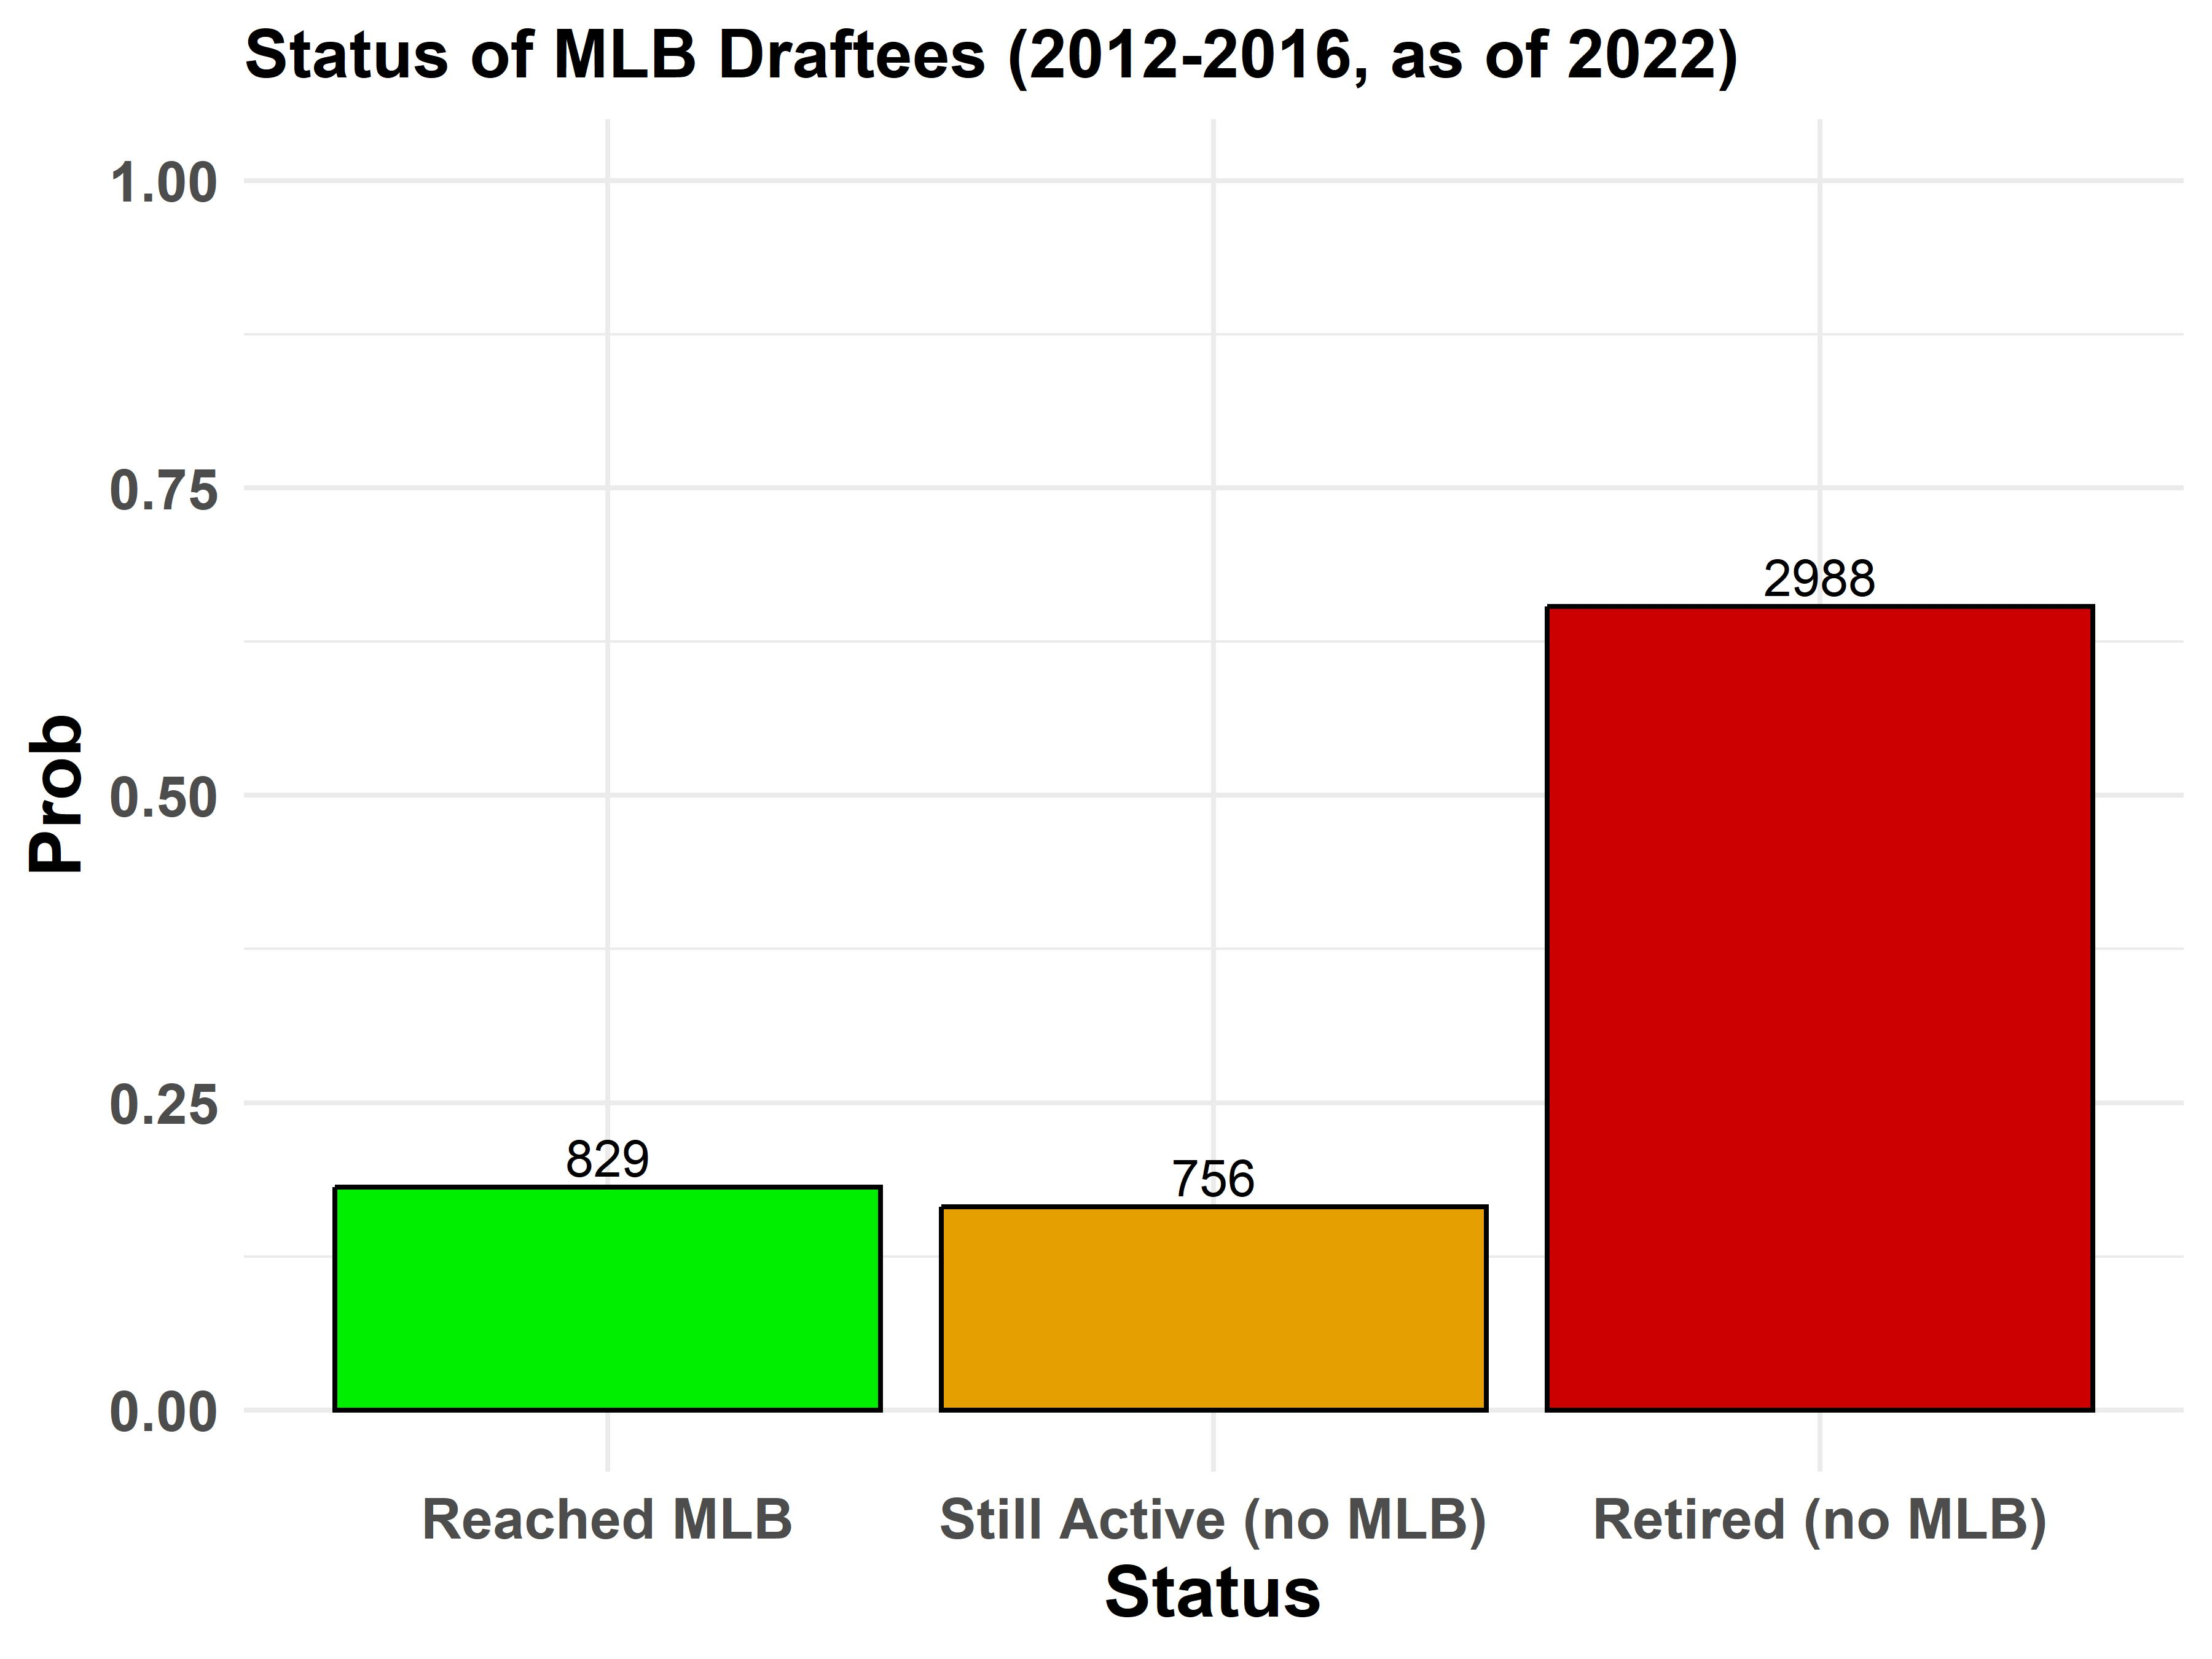
\includegraphics[width=0.75\linewidth]{descplot2}
        \end{tikzfigure}

        \hide{This is the best thing I can think of to get it so that my plots are kitty corner from each other, though it seems like there should really be a better way, I am running out of patience with latex. At the very least, this seems to be working so that I can make the poster seem to be a little bit better organized, though I regret the ample amount of whitespace.}

        \begin{tikzfigure}[Positions and types of drafted players.]
            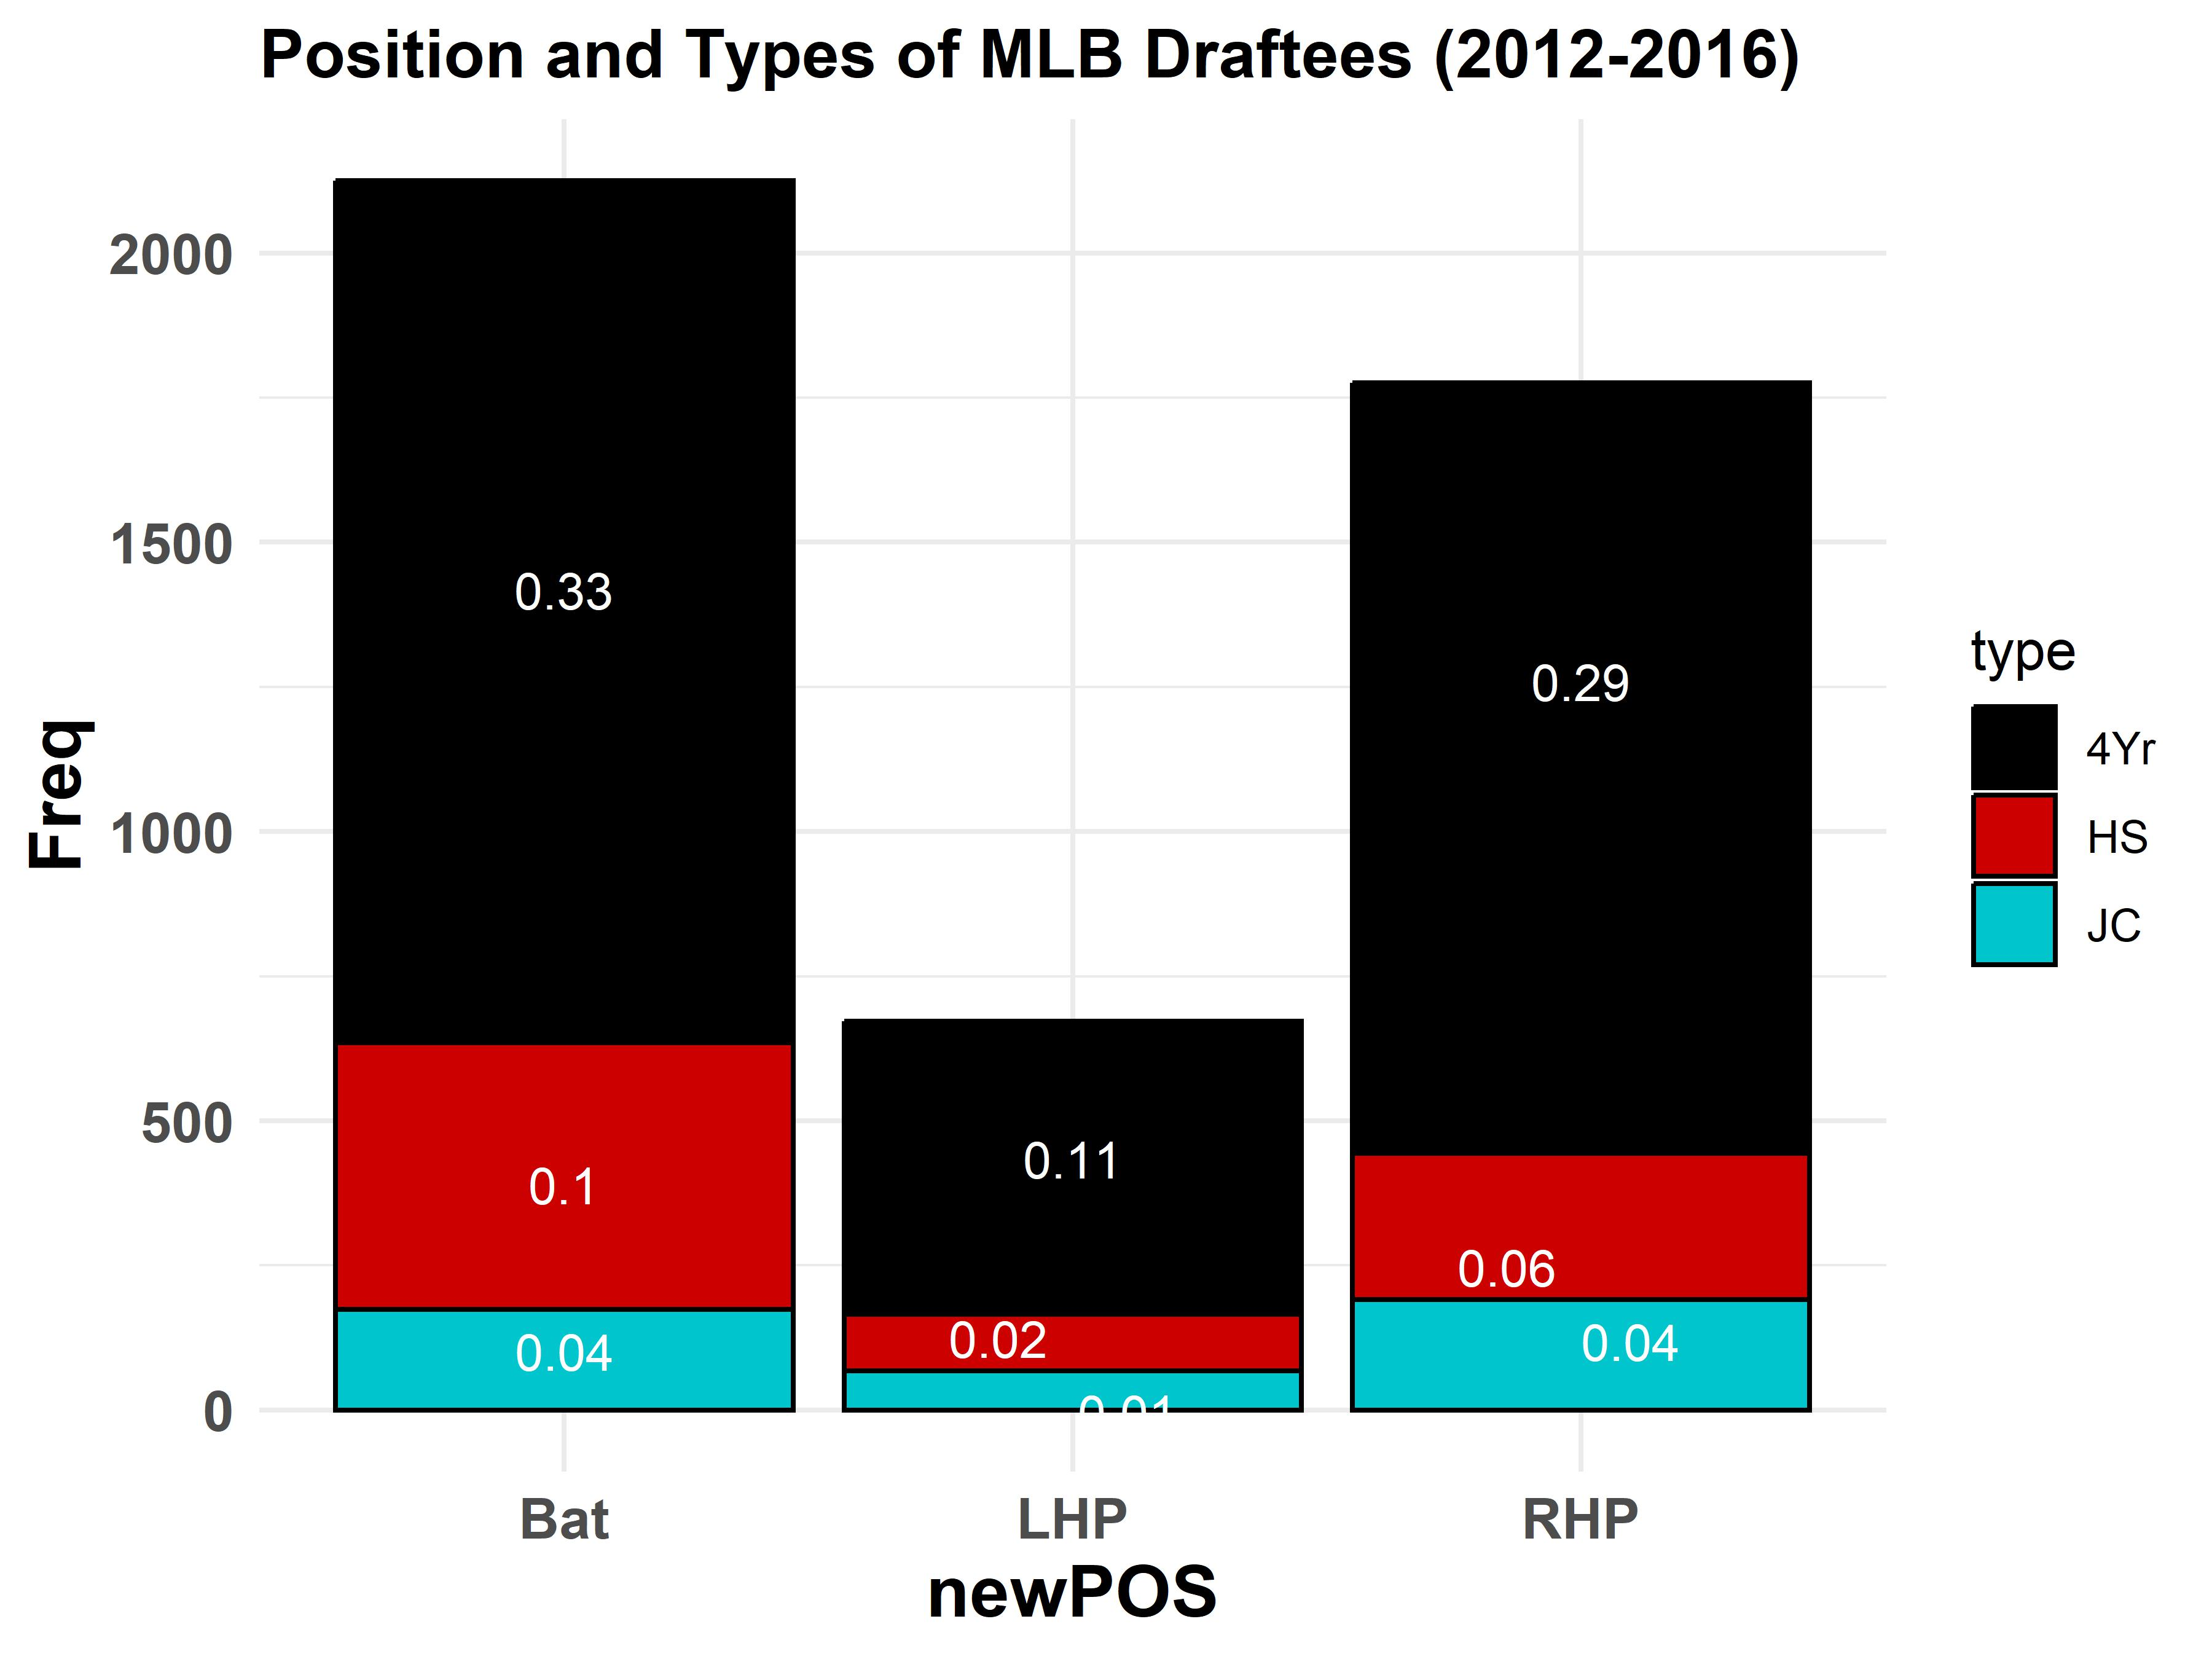
\includegraphics[width=0.75\linewidth]{descplot3}
        \end{tikzfigure}
             
         \end{multicols}
         
    }

    \column{0.36}
    \block{Methodology}{
        \lipsum[4]
        \begin{equation*}
           p(\theta|y) \propto p(y|\theta)p(\theta) 
        \end{equation*}
        \begin{center}
        \captionof{Eq. 1: }{A famous equation}            
        \end{center}
        \lipsum[11]
    }
    
    \block{Results}{
        In this section, focus on plots (maybe 3-4 below) and then a short, digestible list of key takeaways. Not too much text! \lipsum[13]
        
        %\vspace{.25em}
        % \begin{tikzfigure}[Predicted risks of Reaching MLB and Retiring for first round (average bonus) Batters]
        %     \includegraphics[width=0.465\linewidth]{Batter_MLB_Rnd1_AvgBon.jpg}
        %     %\includegraphics[width=0.325\linewidth]{LHP_MLB_Rnd1_AvgBon.jpg}
        %     %\includegraphics[width=0.325\linewidth]{RHP_MLB_Rnd1_AvgBon.jpg}
        %     \includegraphics[width=0.465\linewidth]{Batter_Retire_Rnd1_AvgBon.jpg}
        %     %\includegraphics[width=0.325\linewidth]{LHP_Retire_Rnd1_AvgBon.jpg}
        %     %\includegraphics[width=0.325\linewidth]{RHP_Retire_Rnd1_AvgBon.jpg}
        % \end{tikzfigure}
        % \vspace{.25em}
        
        %\vspace{.25em}
        \begin{tikzfigure}[Predicted risks of Reaching MLB and Retiring across picks (average bonus) for LHP]
            %\includegraphics[width=0.45\linewidth]{Batter_MLB_byPick_AvgBon.jpg}
            \includegraphics[width=0.49\linewidth]{LHP_MLB_byPick_AvgBon.jpg}
            %\includegraphics[width=0.325\linewidth]{RHP_MLB_byPick_AvgBon.jpg}
            %\includegraphics[width=0.45\linewidth]{Batter_Retire_byPick_AvgBon.jpg}
            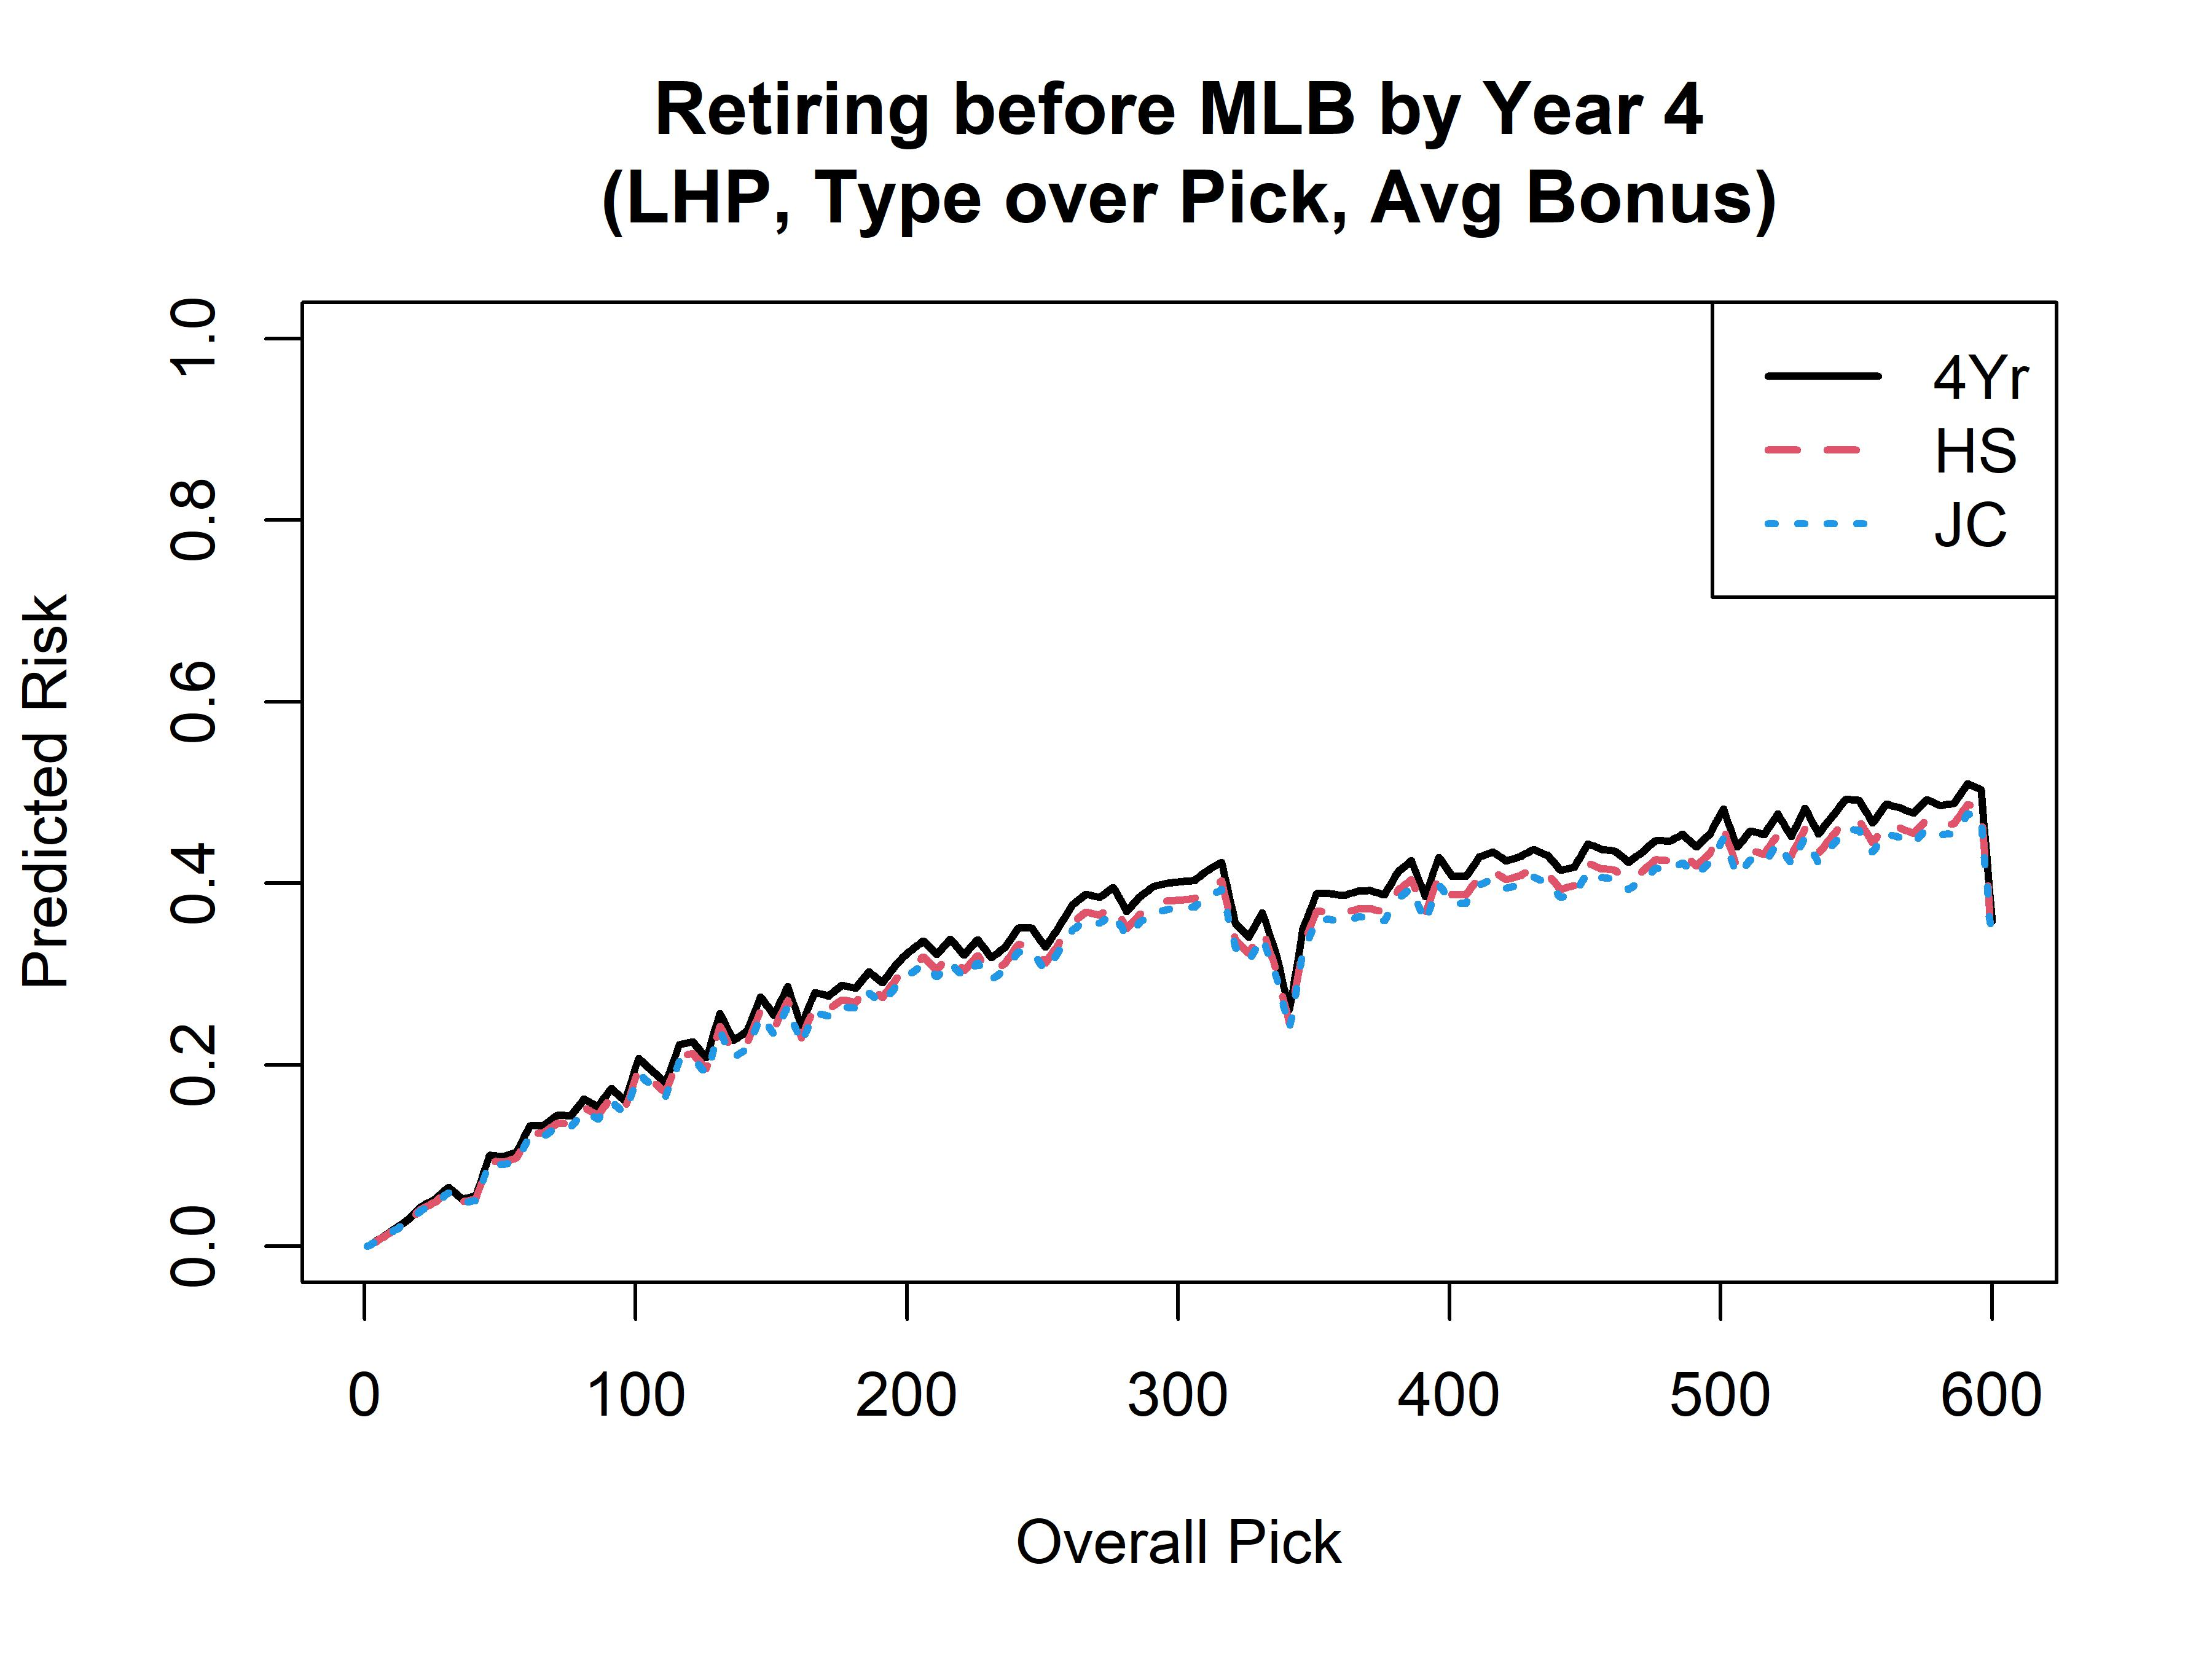
\includegraphics[width=0.49\linewidth]{LHP_Retire_byPick_AvgBon.jpg}
            %\includegraphics[width=0.325\linewidth]{RHP_Retire_byPick_AvgBon.jpg}
        \end{tikzfigure}
        \vspace{.25em}
        
        %\vspace{.25em}
        \begin{tikzfigure}[Predicted risks of Reaching MLB for HS RHP across Round and Bonus]
            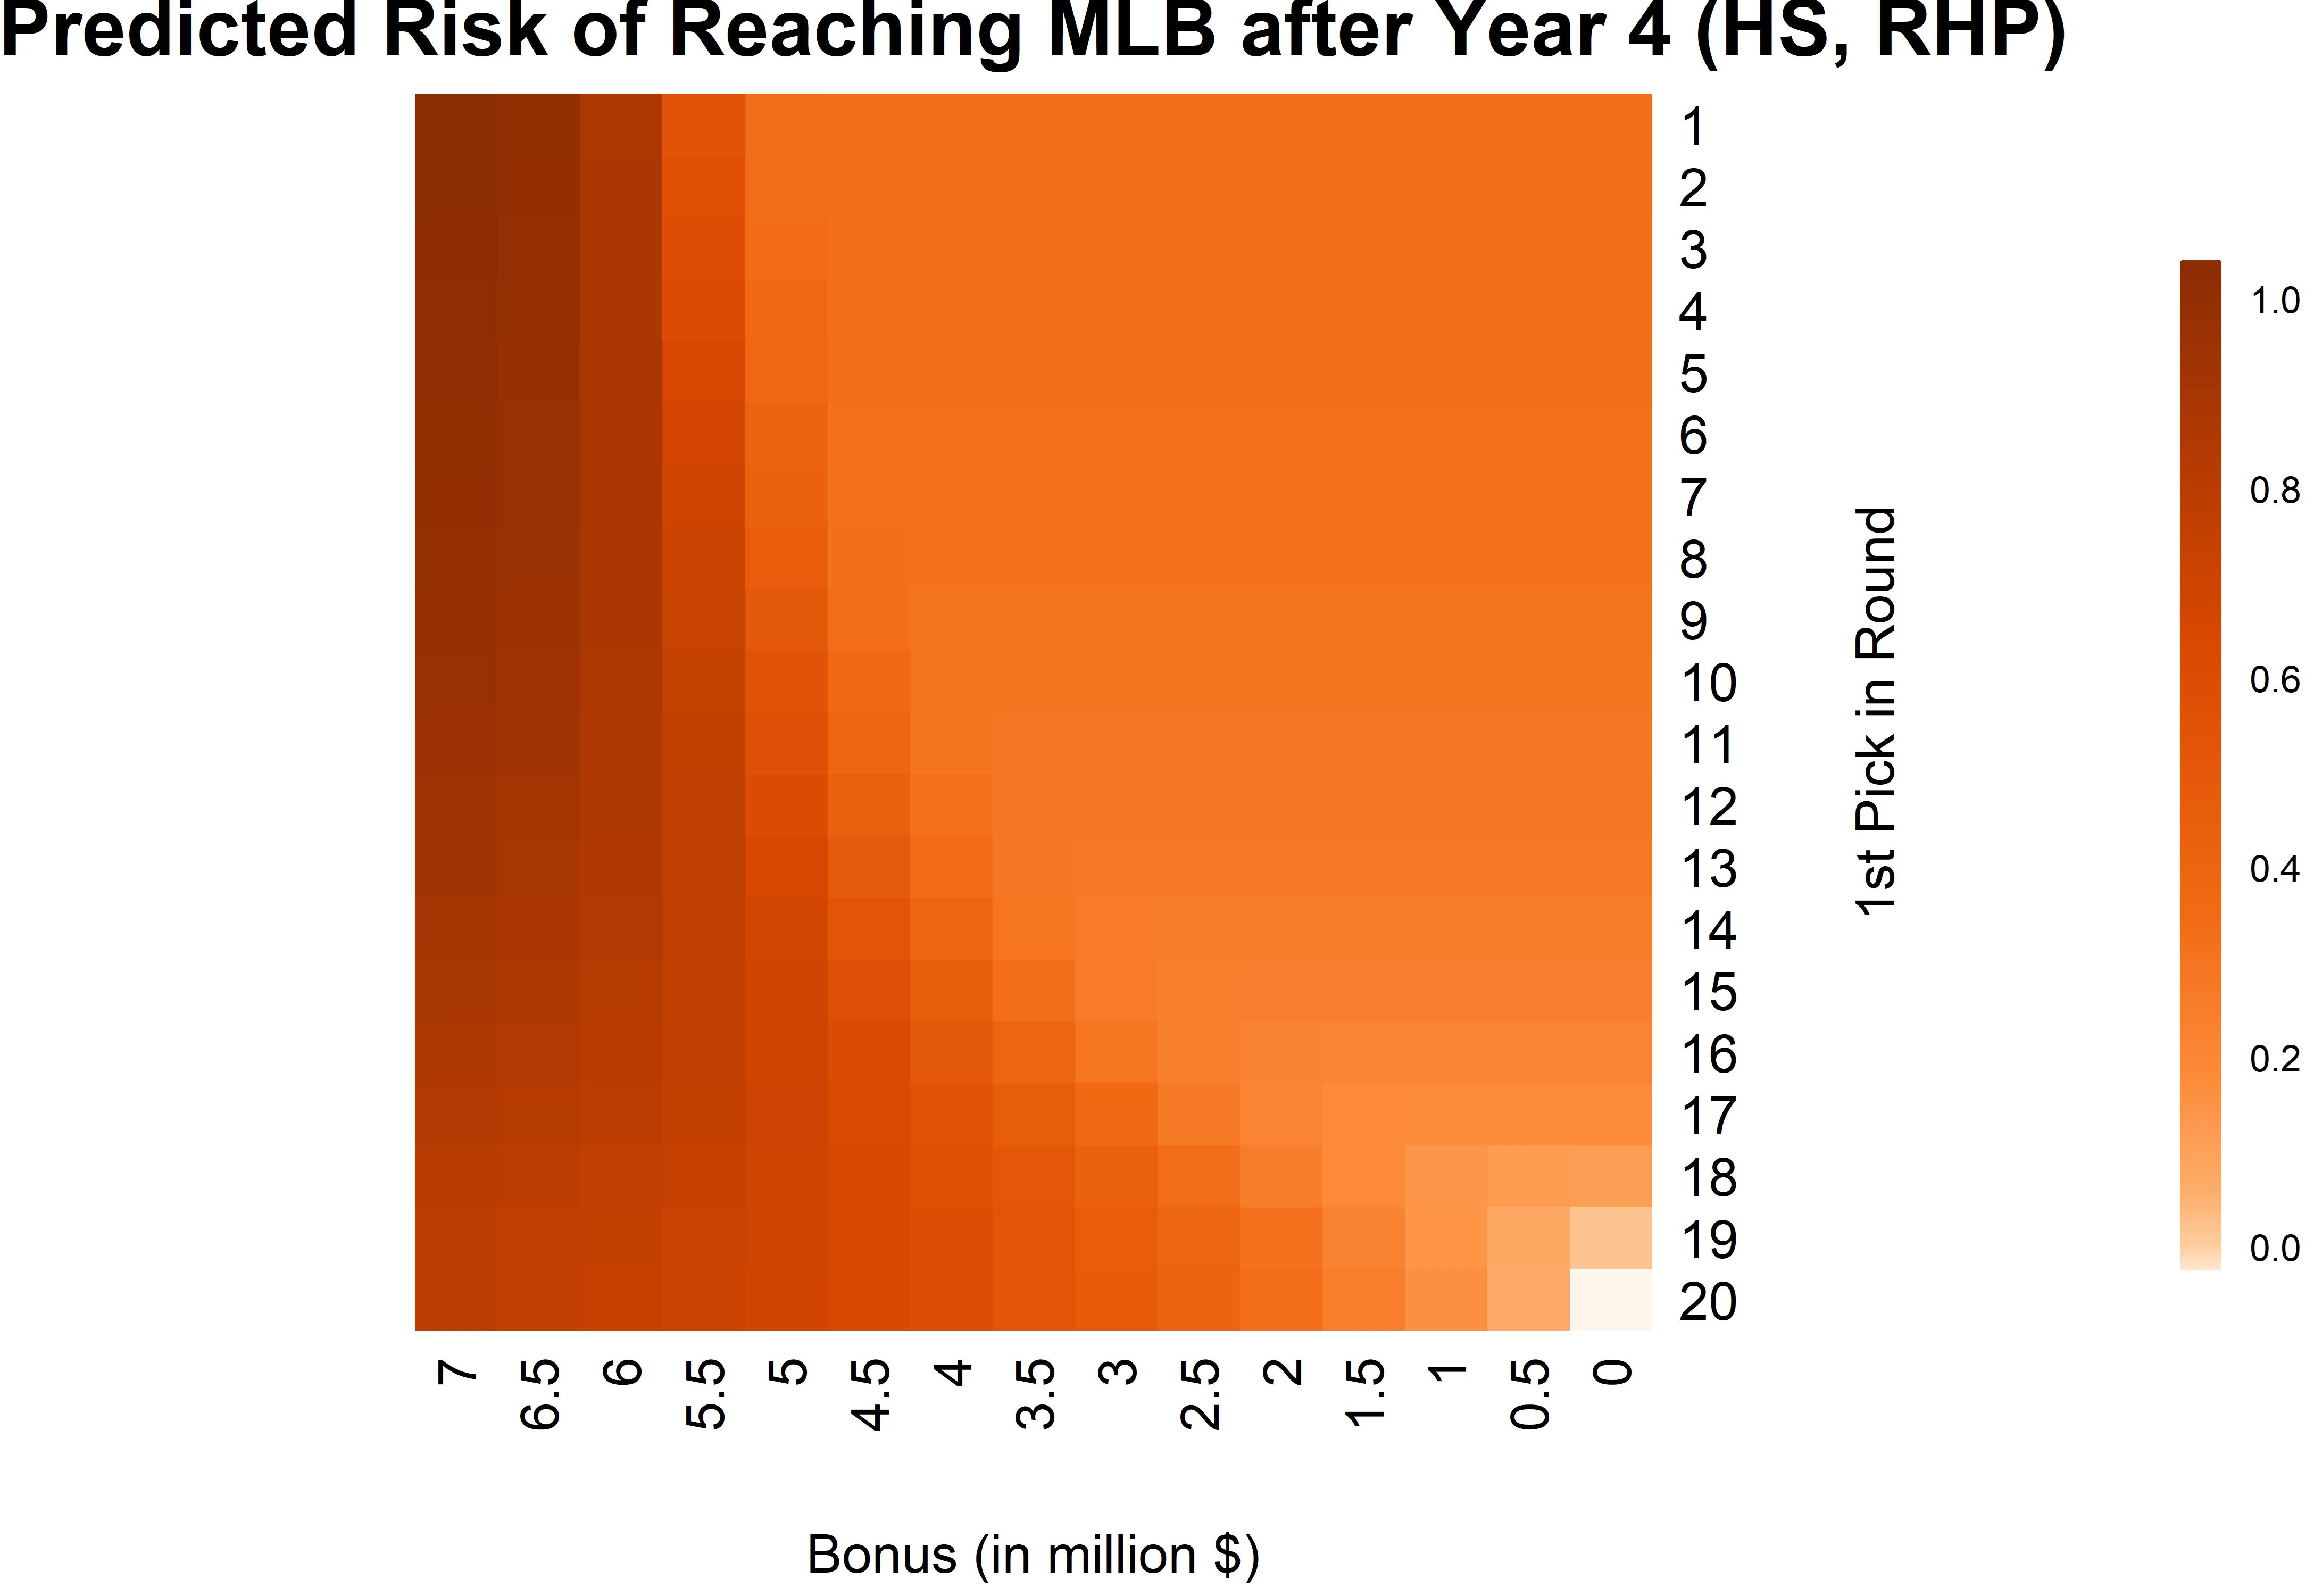
\includegraphics[width=.45\linewidth]{HSRHP_OvPckBonus_1pick.jpg}
        \end{tikzfigure}
        \vspace{.25em}

        Other notable results:

        \begin{itemize}
            \item Notable result 1
            \item Notable result 2
            \item  Notable result 3 and how it is related/different from the literature \cite{Pifer:2020jse}
        \end{itemize}

    }

    \column{0.32}
    \block{Discussion/Future Work/Web App}{
        \lipsum[8]

%        \begin{multicols}{2}
        \begin{tikzfigure}[Maybe a screenshot of the app, or the most relevant result plot.]
            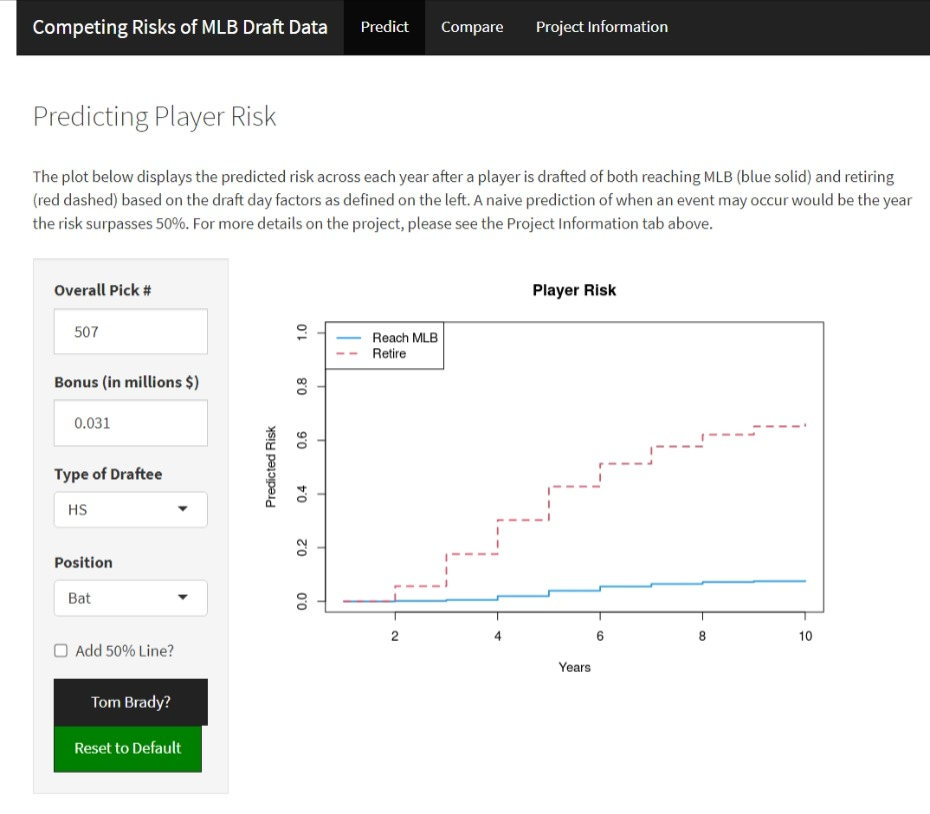
\includegraphics[width=.65\linewidth]{app_example.jpeg}
        \end{tikzfigure}
        
        \begin{center}
            
\includegraphics[width = .065\textwidth]{qr-code.png}
        \end{center}
 %       \end{multicols}

        \lipsum[9]

    }
    
    
    \block{References}{
        Only if needed.\\
        \begin{footnotesize}
        \printbibliography[heading=none]
        \end{footnotesize}
    }
\end{columns}
\end{document}